\begin{figure}[htbp]
\section*{ ZMYM3}
\centering
\begin{subfigure}[b]{0.95\textwidth}
\centering
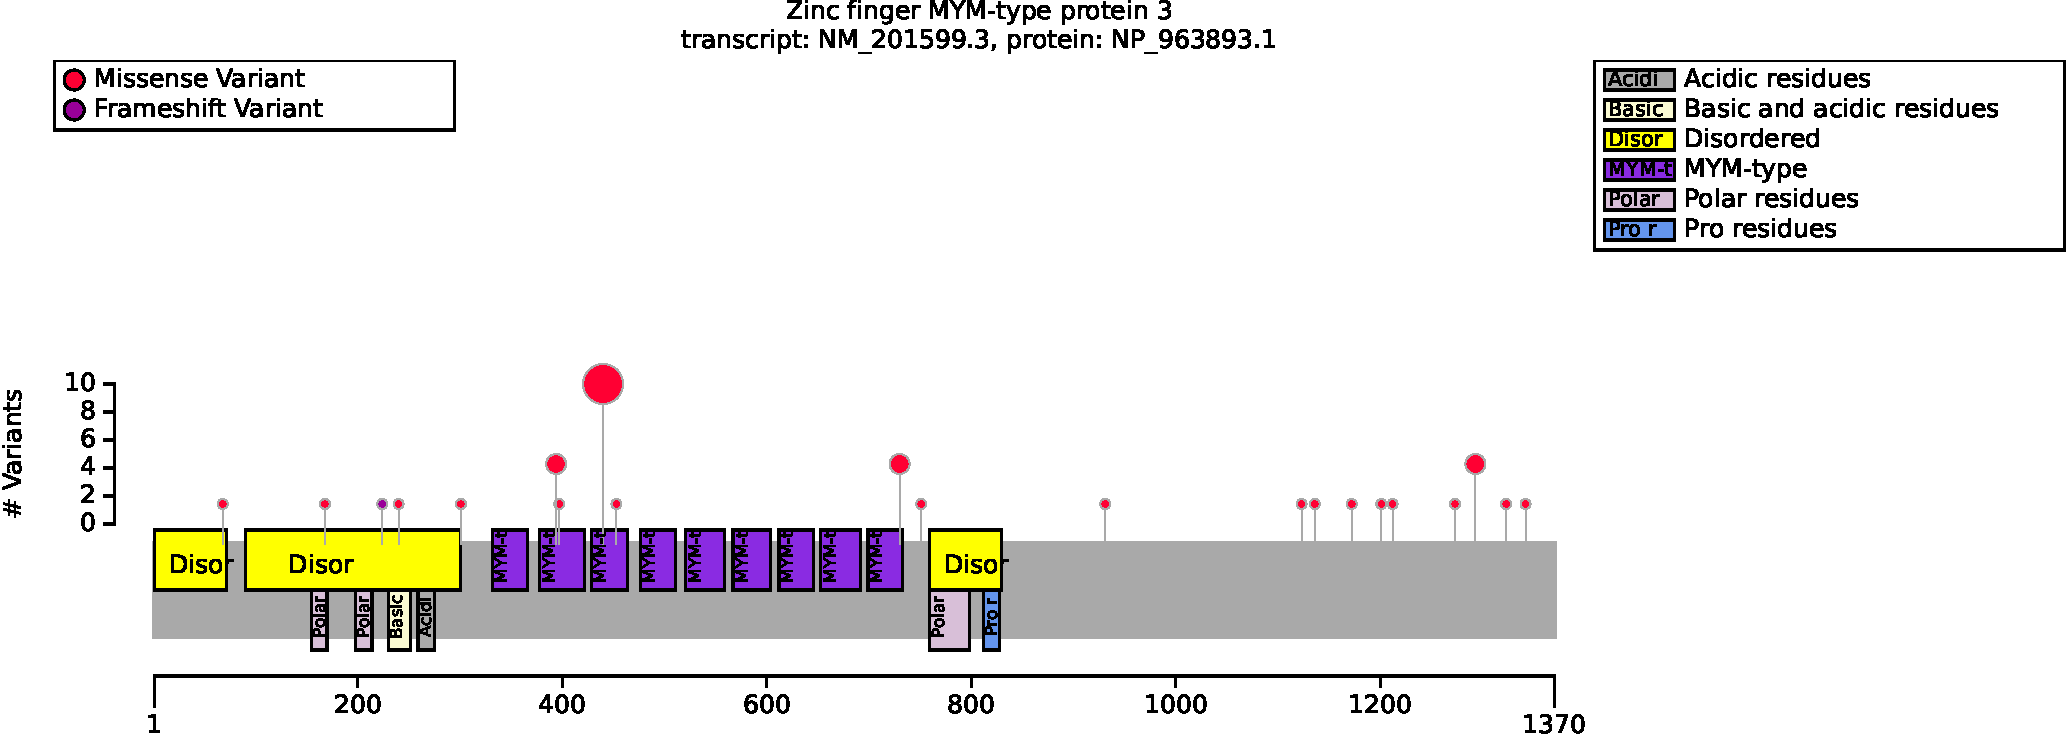
\includegraphics[width=\textwidth]{ img/ZMYM3_protein_diagram.pdf} 
\captionsetup{justification=raggedright,singlelinecheck=false}
\caption{Distribution of variants in ZMYM3}
\end{subfigure}

\vspace{2em}

\begin{subfigure}[b]{0.95\textwidth}
\centering
\resizebox{\textwidth}{!}{
\begin{tabular}{llllrr}
\toprule
Genotype (A) & Genotype (B) & total tests performed & significant results\\
\midrule
N term & other & 9 & 0\\
R441 & other & 9 & 0\\
\bottomrule
\end{tabular}
}
\captionsetup{justification=raggedright,singlelinecheck=false}
\caption{Fisher Exact Test performed to compare HPO annotation frequency with respect to genotypes.}
\end{subfigure}

\vspace{2em}

\caption{The cohort comprised 29 individuals (3 females, 26 males). A total of 41 HPO terms were used to annotate the cohort. Disease diagnosis: Intellectual developmental disorder, X-linked 112 (OMIM:301111). No statistically significant results identified. A total of 29 unique variant alleles were found in \textit{ZMYM3} (transcript: \texttt{NM\_201599.3}, protein id: \texttt{NP\_963893.1}).}
\end{figure}
